\documentclass[twocolumn, 10pt, a4paper]{article}

% standard packages
\usepackage{titlesec, blindtext, color}                                  % standard packages
\usepackage[usenames,dvipsnames,svgnames,table]{xcolor} % extra colors 
\usepackage{graphicx}                                                       % figures
\usepackage{natbib}                                                          % bibliography
\usepackage[english]{babel}                                              % correct hyphenation (afbreekstreepjes)
\usepackage{booktabs}                                                     % for midrule in tables
\usepackage{rotating}                                                        % for sdeways table

% PAGE MARGINS
\usepackage[top=2.5cm, bottom=2.5cm, left=2cm, right=2cm]{geometry}

% FONT
\usepackage[lf]{berenis}
\renewcommand*\familydefault{\sfdefault} 
\usepackage[T1]{fontenc}
% for other fonts, and how to install them, see the LaTeX Font Catalogue:
% http://www.tug.dk/FontCatalogue/

% LINE SPACE
\linespread{1.1}                          % more space between lines
\setlength{\parindent}{5mm}       % indenting first line paragraph


% HYPHENATION (afbreekstreepjes)
% set words that are not abbreviated correctly  (expand list when necessary)
\hyphenation{catch-ment areas a-na-lyse}


%%%%%%%%%%%%%%%%%%%%%%%%%%%%%%%%%
%%%%%%%%%%%%%%%%%%%%%%%%%%%%%%%%%
% START
%%%%%%%%%%%%%%%%%%%%%%%%%%%%%%%%%
%%%%%%%%%%%%%%%%%%%%%%%%%%%%%%%%%

\begin{document}

\title{\vspace{-1cm}\Huge{Data analysis and/or modelling\\
of some hydrologic phenomenon}}
\author{\Large{My Name}}
\date{\normalsize{MSc thesis proposal\\
Hydrology and Quantitative Water Management Group,
Wageningen University}}

\maketitle

\section{Problem description}

Remove text from this template and write your own (of course). Feel free to change headers, but make sure the topics are covered. There is a lot of valuable information available on the internet on how to write thesis proposals and the thesis reports themselves. 

In this Section, you should:
\begin{itemize}
\item Motivate and justify the research. Put your research in global context (who cares about your research?)
\item State what has been done already. Summarize relevant literature \citep{Brauer2011}.
\item State what has NOT been done yet. Where is the gap in knowledge? This should lead directly to the research objectives in the next Section.
\end{itemize}
  
\section{Research objectives}

State objectives clearly. What is the point of this research? The aim should follow directly from the problem description. 

\section{Research questions}

Which questions do you want to answer in order to reach the objectives? Divide into sub-questions for clarity.


\section{Field site and data}

Are you going to use other people's data or collect data yourself? What are the considered locations, instruments, resolutions? You can also include the data in the methods.

\section{Methods}

How are you going to find the answer to your questions? What do you need for this? Describe the core measurement equipment or models briefly. It often helps to link the steps in the methodology to the research questions.


\section{Timetable}

Adapt the Table below to make it specific for your project (or make your own). Set deadlines for the products. Be as specific as possible: mention when you will collect which data /do which model runs / write which parts of the report. It often helps to link activities and products to your sub-questions. A specific planning can help later on to see if you are on schedule or that you should e.g. shorten a certain data-processing step or stop calibrating your model, so you have enough time to do the analyses and answer your research questions. It often helps to link the tasks to the methodology (and therefore to the research questions). Specify special conditions: are you planning to take courses, vacation, etc. 


% table with schedule
\begin{table*}[t]
	\caption{Schedule of the project.}
	\label{tab:schedule}
	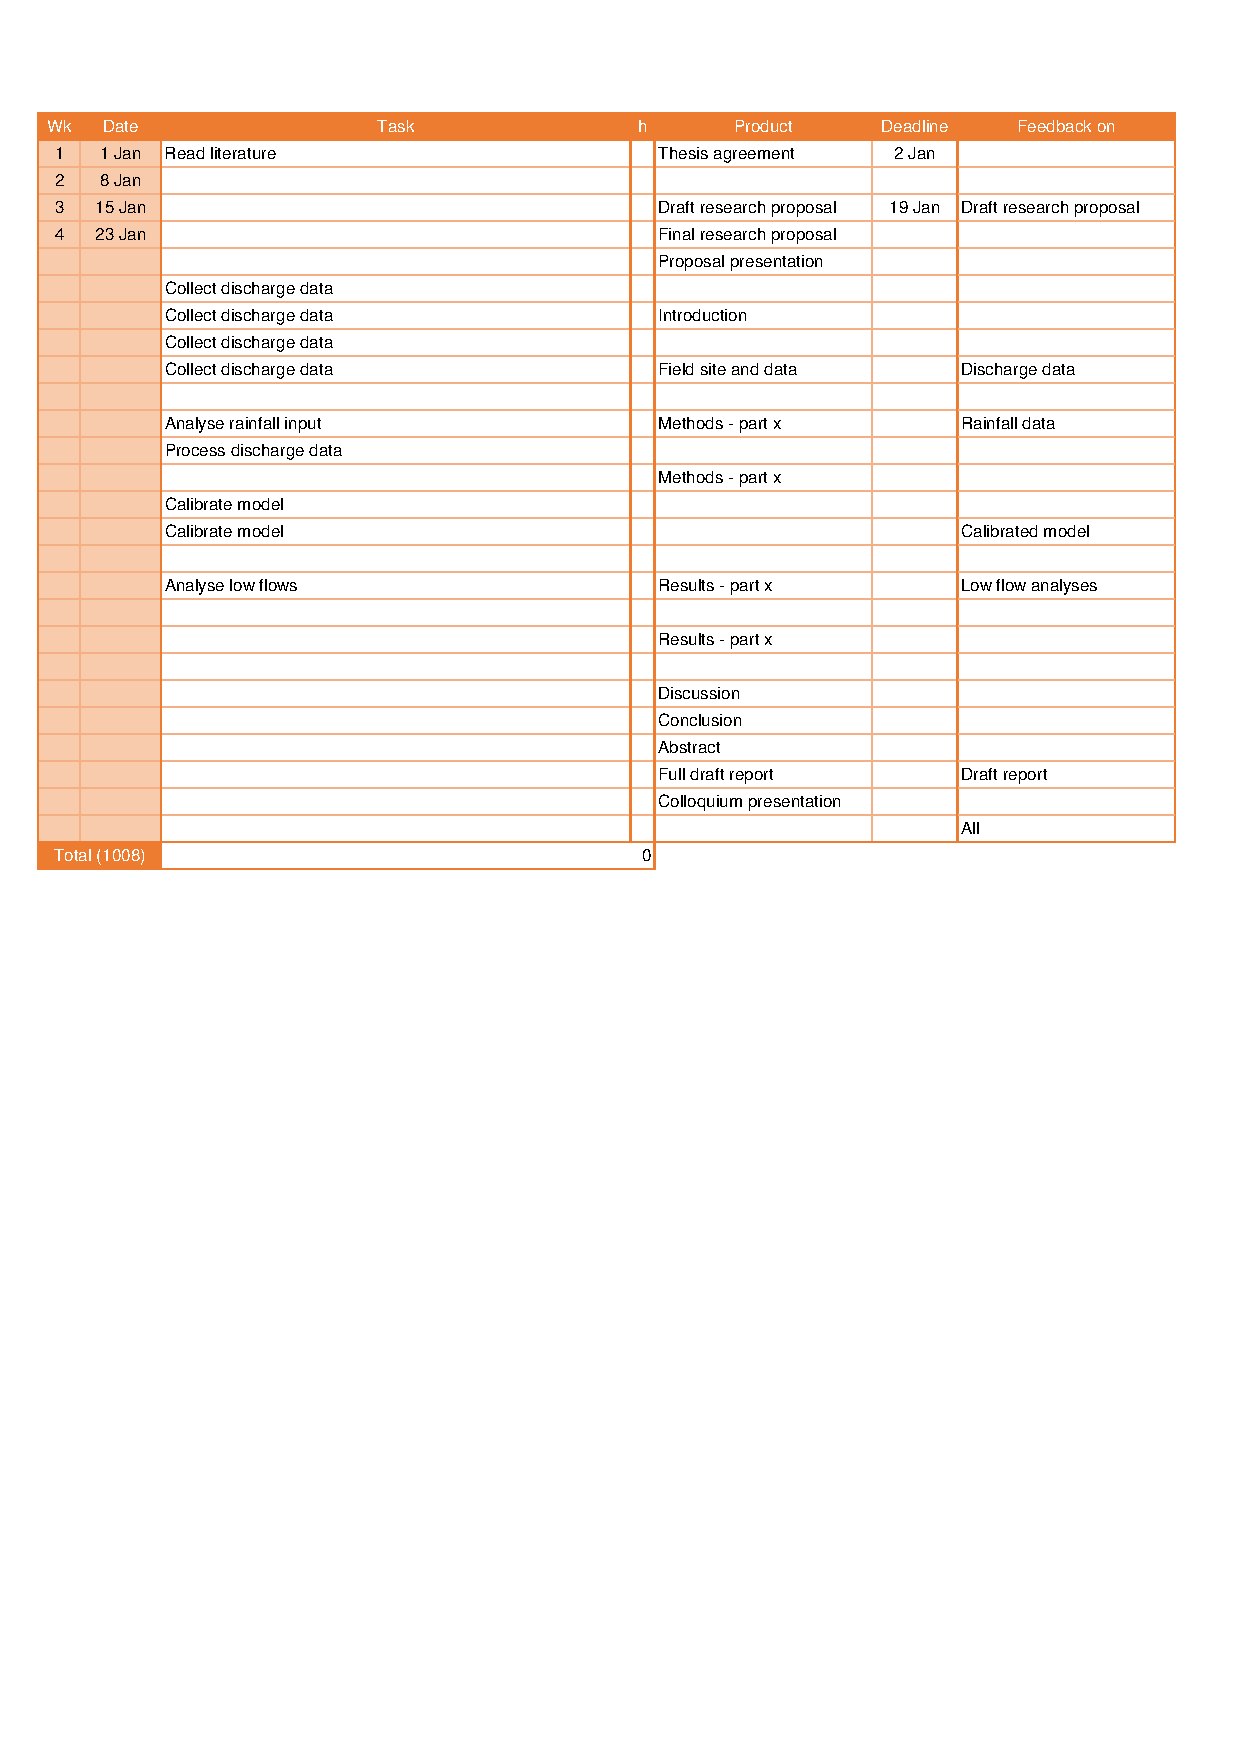
\includegraphics[width=2.1\columnwidth, trim=5mm 80mm 5mm 18mm, clip=true]{figs/thesis_planning.pdf}
\end{table*}
% If not the whole table is shown: adjust the numbers behind "trim". 
% Those are the cropped sides in the order left - bottom - right - top.




%%%%%%%%%%%%%%%%%%%%%%%%%%%%%%%%%
% BIBLIOGRAPHY
%%%%%%%%%%%%%%%%%%%%%%%%%%%%%%%%%

\renewcommand{\bibname}{Bibliography} 
\bibliographystyle{elsart-harv}
\bibliography{references_thesis}

% to add items to the bibliography:
% option 1. open "references_thesis.bib" in JabRef (free downloadable), enter more papers
% option 2. open "references_thesis.bib" in NotePad, go to Google Scholar, find paper, click "cite", click "import into BiBTeX", copy text into NotePad



%%%%%%%%%%%%%%%%%%%%%%%%%%%%%%%%%
% END
%%%%%%%%%%%%%%%%%%%%%%%%%%%%%%%%%


\end{document}
